\documentclass[12pt]{rockefeller}
\usepackage[pdftex]{graphicx} 
\graphicspath{{./figures/}} %directory of figures
\usepackage[english]{babel} %set language
\usepackage{helvet} %set font to Helvetica
\renewcommand\familydefault{\sfdefault} %set font to Helvetica
\usepackage{fancyhdr} %header and footer
\usepackage[utf8]{inputenc} %allow greek input
\usepackage[LGR,T1]{fontenc} %allow greek input
\newcommand{\textgreek}[1]{\begingroup\fontencoding{LGR}\selectfont#1\endgroup} %allow greek input
\usepackage{enumerate}
\usepackage{subcaption}
\usepackage{tabu}
\renewcommand\thesubfigure{\alph{subfigure}}
\usepackage{color,soul}
\usepackage[labelfont=bf]{caption} 
\usepackage{hyperref} %allow hypertexting
\usepackage[acronym,xindy,toc]{glossaries} %glossary 
\makeglossaries %glossary 
\usepackage[xindy]{imakeidx} %glossary 
\makeindex %glossary 
\usepackage[backend=biber,style=nature,]{biblatex}
\bibliography{./tasos_v2.bib}

%\usepackage{enumerate}
%\usepackage{threeparttable}
%\usepackage{multirow}
%\usepackage[algoruled,linesnumbered,lined]{algorithm2e}
%\usepackage[font=footnotesize,caption=false]{subfig}
%\usepackage{amssymb}
%\usepackage{amsmath}
%\usepackage[pdftex,bookmarks=true]{hyperref}
%\newcommand{\subsubsubsection}[1] {\noindent {\underline {#1}}}
\newcommand{\snp}[1] {\noindent {\underline {#1}}}
\newcommand{\cyan}[1]{\colorbox{cyan}{#1}}

\begin{document}

\author{Tasos Gogakos}
\title{\MakeUppercase{Characterizing human transfer rnas by hydro-trnaseq and par-clip}}
\date{June 2017}

\maketitle

\thispagestyle{empty}
\makecopyright


\begin{abstract}

The participation of \glspl{trna} in \gls{test} fundamental aspects of biology and disease necessitates an accurate, experimentally confirmed annotation of tRNA genes, and curation of precursor and mature tRNA sequences. This has been challenging, mainly because RNA secondary structure and nucleotide modifications, together with tRNA gene multiplicity, complicate sequencing and sequencing read mapping efforts. To address these issues, we developed hydro-tRNAseq, a method based on partial alkaline RNA hydrolysis that generates fragments amenable for sequencing. To identify transcribed tRNA genes, we further complemented this approach with Photoactivatable Crosslinking and Immunoprecipitation (PAR-CLIP) of SSB/La, a conserved protein involved in pre-tRNA processing. Our results show that approximately half of all predicted tRNA genes are transcribed in human cells. We also report predominant nucleotide modification sites, their order of introduction, and identify tRNA leader, trailer and intron sequences. By using complementary sequencing-based methodologies we present a human tRNA atlas, and determine expression levels of mature and processing intermediates of tRNAs in human cells.
\end{abstract}


%Dedication
\chapter*{} %blank chapter, no title, not included in table of contents
\addtocounter{page}{2} %fix numbering
\vspace{3in} %start the dedication close to the bottom of page
\begin{flushright} %center everything
\emph{\textgreek{Stous gone'is kai ton aderf'o mou}}
\end{flushright}

\chapter*{Acknowledgments} %uncounted chapter

First, I would like to thank my  

\chapter*{contents}
\renewcommand\contentsname{Table of Contents}
\tableofcontents
\cleardoublepage
\phantomsection
\addcontentsline{toc}{chapter}{List of Figures}
\listoffigures
\cleardoublepage
\phantomsection
\addcontentsline{toc}{chapter}{List of Tables}
\listoftables

%glossary
\newacronym[plural=tRNAs, firstplural=transfer RNAs]{trna}{tRNA}{transfer RNA}
\newacronym{test}{tEsT}{test2}
\newacronym{ncrna}{ncRNA}{noncoding RNA}
\chapter*{Glossary}
\printglossary[type=\acronymtype,nonumberlist,title={List of Abbreviations}]

%----------
%mainmatter
%----------
\mainmatter
\pagestyle{fancy}
\fancyhf{}
\lhead{\chaptername\ \thechapter}
\rhead{\thesection}
\rfoot{\thepage}

\chapter{Introduction}
\section{Overview}
Transfer RNAs (tRNAs) are essential factors for the expression of genetic information, serving as the adaptor molecules that decode the genetic code during protein synthesis \hl{cite Crick tie club letter}, and are among the earliest studied \gls{ncrna} non-coding RNA molecules \cite{Woese:1967, Soll:1995}. Despite their highly conserved participation in the translational machinery, there is growing evidence that they play roles in other cellular processes, including non-coding RNA-mediated gene silencing and responses to cellular stress. The biological importance of tRNAs and their associated proteins is underscored by the pathologic conditions that are related to aberrations in their expression and function or The biological significance of tRNAs and their protein interactions is underscored by the number of human diseases caused by mutations in tRNAs and tRBPs \hl{8,11-15 from TRP}. 



Yet, in recent years tRNAs received new attention in the context of codon-resolved translational control \cite{Dana:2012kq,Dana:2014bs,Mahlab:2012dg,Plotkin:2010fu,Tuller:2010ge,Weinberg:2016kh}, and due to the involvement of their metabolic byproducts in regulation and cross-talk with processing and effector functions of other classes of non-coding RNAs (ncRNAs) \cite{Hasler:2016ce,Ivanov:2011iu,Lee:2009fb}. Nevertheless, the lack of reliable methods for tRNA quantification has hampered such analyses, and necessitated the use of predicted tRNA gene copy number as a surrogate index of expression \cite{Iben:2014dt,Pechmann:2012ey,Tuller:2010ge}. This hinged on the assumption that predicted tRNA gene loci are all expressed constitutively and equally, even though there has been experimental evidence against it \cite{Gingold:2014iz}. Similarly, experimental tRNA gene annotation in the past had to focus on RNA polymerase III (POLR3) ChIP-seq \cite{Kutter:2011ff} \cite{Moqtaderi:2010hc} \cite{Oler:2010fb} or hybridization-based approaches \cite{Dittmar:2004fb} \cite{Goodarzi:2016gd}. The former, however, were impeded by their restricted genomic resolution and the assumption that POLR3 binding always leads to productive tRNA expression followed by complete processing, while the latter fell short of providing absolute counts and did not address the discovery of new transcripts and genes, assuming also normal hybridization rules for modified nucleosides.

An improvement in tRNA quantification has arisen from recent efforts that employed modification-reverting enzymes prior to sequencing, in order to minimize stalling of reverse transcriptase at modified sites \cite{Cozen:2015ds} \cite{Zheng:2015dw}. However, an extensive annotation of human genes and transcripts was foregone because the focus was either on mature tRNAs only \cite{Zheng:2015dw} or on tRNA fragments not inclusive of full-length precursor tRNA (pre-tRNA) transcripts \cite{Cozen:2015ds}. Thus, to-date an experimentally validated list of curated mature and pre-tRNA sequences and annotating tRNA genes in human is still missing.

We have combined complementary high-throughput techniques for obtaining the sequence composition and abundance of tRNAs in human embryonic kidney cells (HEK293). We developed hydro-tRNAseq, a modified small RNA sequencing protocol based on partial alkaline hydrolysis of input RNA, in order to identify and quantify tRNAs, and provided evidence for the validity of this approach when determining the accumulation of disease-associated tRNA intron fragments caused by mutations in the tRNA splicing machinery \cite{Karaca:2014em}. Here we extend this approach by applying it to tRNA-enriched size fragments with the aim to annotate and curate all tRNAs. Since tRNA processing, such as precursor trimming and intron removal, is a fast process\cite{Foretek:2016ea}, we also aimed to enrich specifically for pre-tRNAs in order to identify and annotate the corresponding unique tRNA gene template. Thus, we performed PAR-CLIP on SSB, a conserved and ubiquitous protein involved in 3’ tRNA processing \cite{Bayfield:2009cx} \cite{Bayfield:2010cs} \cite{Stefano:1984wp}. 

\subsection{tRNA biogenesis}
tRNA genes are transcribed by RNA polymerase III \cyan{(POLR3)} that uses promoters internal to the DNA sequence of the tRNA gene (tDNA). The primary transcript is a precursor tRNAs \cyan{(pre-tRNA)} with a 5' triphosphate. In humans, a minority of tRNA transcripts \hl{(see section XXX)} harbor introns. A dedicated tRNA splicing complex composed fo core and accessory proteins carries out tRNA splicing \hl{cite references}. Pre-tRNAs comprise the mature tRNA sequence, and 5' leader and 3' trailer extensions, which are trimmed in a coordinated manner by endonucleases and other processing factors. The ribonucleoprotein \cyan{(RNP)} complex RNase P removes the 5' leaders, leaving a 5' monophospahte, and ELAC2, the human homolog of tRNase Z trims the 3' trailer, leaving a 3' hydroxyl \cyan{(OH)}. Next, the universally conserved 3' terminal CCA tail is added by TRNT1, the tRNA nucleotidyll transferase 1 \cyan{(TRNT1)}, and acts as the acceptor of the amino acid. tRNAs are further modified by chemical nucleotide modifications \hl{(see section XXX)}, exported from the nucleus to the cytoplasm where they can undergo further modifcations, are aminoacylated with their cognate amino acid by aminoacyl tRNA synthetases, and are finally presented to the ribosome by translation factors to participate in protein synthesis Fig. \ref{biogenesis}. \hl{cite 16,17 from TRP}

Although these processes allow for multiple levels of regulation, variation in tRNA expression across tissues or between normal and pathologic conditions has not been studied extensively, mainly for two reasons. First, until recently there was the assumption that their essentiality obviated a need for any specialized transcriptional or post-transcriptional control. Second, the lack of an extensively curated and experimentally validated tRNA profile prevented quantitative and systematic studies. Nevertheless, it is now clear that the expression of tRNAs can be dynamic and can indeed exhibit tissue specificity1 \hl{18 from TRP}. Importantly, abnormal tRNA expression levels have been correlated and causally associated with pathologic conditions, such as cancer \hl{14 from TRP}.
\newline
\begin{figure}[!ht]%
\centering
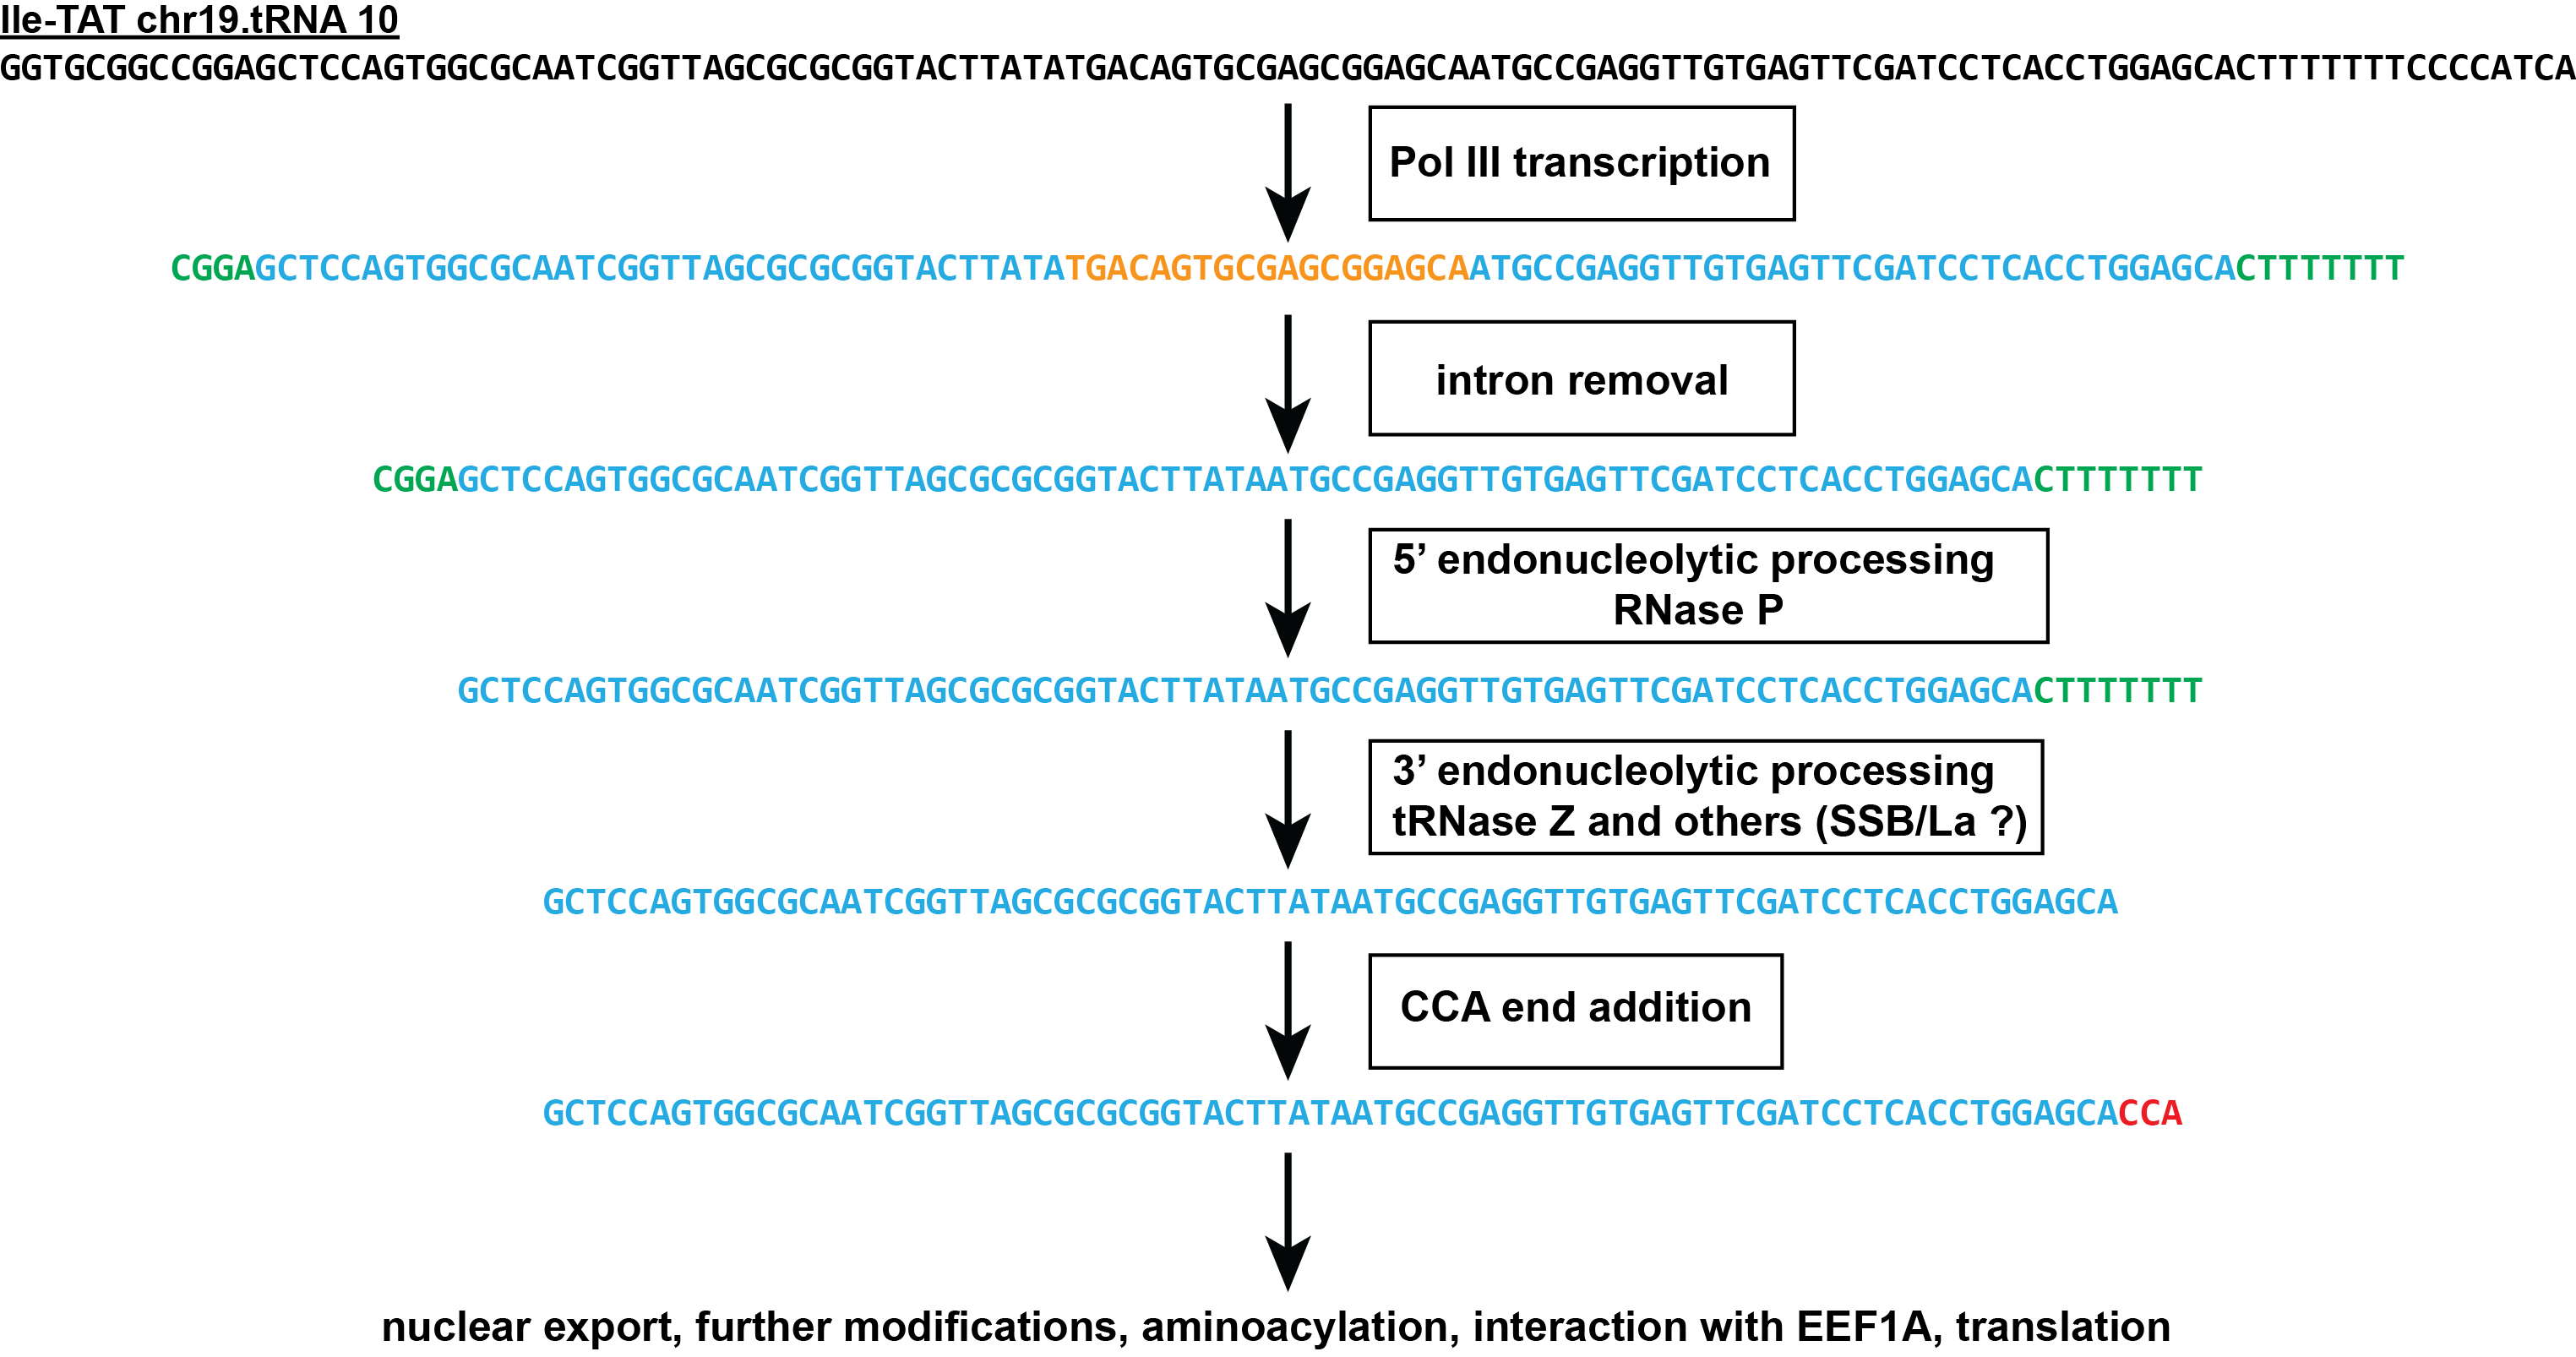
\includegraphics[width=\textwidth]{biogenesis.png}%
\caption[tRNA biogensis]{\textbf{Overview of tRNA biogenesis and processing.} thththt}
%\textbf{\caption{tRNA biogenesis}} 
\label{biogenesis}%
\end{figure}

\subsection{tRNA sequencing}
Evidently the biogenesis pathway of tRNAs is quite a complex one. 
Already some of the possible problems associated with tRNA annotation become apparent. 
Issues that complicate tRNA sequencing and analysis pertain to both experimental and bioinformatic problems:
A) Experimental:%\begin{enumerate}[label=\Alph*]
\vspace{-2.5mm}
\begin{enumerate}[i)]
\itemsep-0.5em 
\item stable 2o and 3o structures. The highly structured tRNA impede ligation steps employed in traditional protocols of small RNA sequencing.
\item extensive post-transcriptional processing. The extensive chemical modification of nucleosides causes stalls, blocks or errors during reverse-transcription \cyan{RT} steps
\item aminoacylation of the 3' end of tRNAs. The 3' aminoacyl-tRNA bind prevents ligation of adapters at the 3' end of tRNAs
\end{enumerate}

Obtaining an RNA-Seq based atlas of human tRNAs is hindered by multiple obstacles. First, sequencing of tRNAs is technically arduous due to their relatively small size, and their stable structure that proves to be a challenge for enzymes used in cDNA library preparations. Second, numerous (>100) tRNA pseudogenes are interspersed in the human genome19. Third, tRNAs undergo extensive post-transcriptional processing, which involves the removal of the 5’ leader and 3’ trailer sequences of the primary transcript, removal of tRNA introns, addition of the universally conserved 3’ CCA end, and addition of a 5’ guanosine to all histidine tRNAs17. Fourth, tRNAs are subjected to extensive chemical modifications on numerous nucleosides, which are likely to lead to mismatches upon the reverse transcription step of the RNA cloning protocols20,21. Some modifications are universally conserved and required for proper tRNA function (e.g. adenosine to inosine deamination at the wobble position of the anticodon and methylation of adenosine in the TpsiC loop)20,22. Since alignment algorithms cannot tolerate multiple mismatches, it is likely that significant numbers of tRNA reads are excluded even if non-default mapping parameters are used. Fifth, tRNA isoacceptors (tRNA molecules that decode synonymous codons) share a large degree of sequence similarity that makes the distinction between alternative isoacceptors and editing products equivocal. Finally, eukaryotic cells harbor two distinct populations of tRNAs, nuclear and mitochondrial, whose length, structure, genomic organization, and processing differ considerably, and thus call for customized annotation procedures. 	Owing to all these hurdles, the normal genetic makeup and variation of the tRNA population in human cells has not been probed with RNA-Seq tools. Instead information about tRNA sequences and genes comes from bioinformatic predictions19,23. Such approaches take into account base-pair covariance, secondary structure predictions of the classical cloverleaf fold of tRNAs, and the tRNA promoter and termination architecture, and scan the human genome in order to identify sequences that are likely to obtain the typical tRNA structure. These analyses have resulted in the most comprehensive standard for whole-genome, predictive annotation of tRNAs so far, and the sequences they have predicted have been used extensively as bona fide tRNAs23.

Thus, it may come as no surprise that obtaining an accurate annotation of tRNA genes and curation of tRNA transcripts is challenging. 
We wanted to obtain an RNA-seq validated list of human nuclear and mitochondrial tRNA gene, and their processing intermediates
This was my goal. To design a method for seequencing and a 

\subsection{Previous efforts for genome-wide tRNA annotation}

To date, no direct and rigorous experimental validation of tRNA sequences has been carried out. Instead, experimental evidence for tRNA expression has been indirect, through: a) chromatin immunoprecipitation and sequencing (ChIP-Seq) studies focusing on the occupancy of genomic locations by POLR3 and/or its transcription factors and b) tRNA microarrays that use the predicted tRNA sequences as the reference for the creation of array probes42-45. These methods, though, have several limitations. ChIP-Seq, for example, uses chromatin occupancy as a proxy for productive RNA synthesis. Conversely, tRNA microarrays have limited sensitivity and specificity thresholds due to off-target hybridization that is potentiated by nucleoside modifications21, while their dynamic range is considerably narrower than RNA-Seq. Finally, neither method is appropriately equipped to determine definitively precursor tRNAs (pre-tRNAs) or their transcription start and termination sites. This is an important limitation, as pre-tRNA fragments have been associated with neurodegenerative diseases46. 
	To address the lack of a global and unbiased analysis of the human tRNA profile, I will develop an experimental and computational methodology for the generation of a reference tRNA atlas. To overcome existing experimental challenges, I will use a customized RNA-Seq technique (HydroRNAseq). To efficiently analyze the sequencing data in silico, I will develop a systematic and iterative bioinformatics platform.


\subsection{Small RNA sequencing protocol}
First, I applied the protocol that the Tuschl lab had previously developed for sequencing small RNAs \cite{Hafner:2012eaa} (\textbf{Fig. \ref{sRNA}}). The experimental procedure resulting in small RNA cDNA library preparation begins with the ligation of barcoded 3' oligonucleotide adapters, pooling of several multiplexed samples, ligation of a 5' adapter, reverse transcription and \cyan{PCR} amplification, followed by high-throughput Illumina sequencing. The different sequences for the 3' and 5' adapters preserves the strandedness of the original RNA sequence, enhancing ncRNA discovery and curation. 

\begin{figure}[!ht]%
\centering
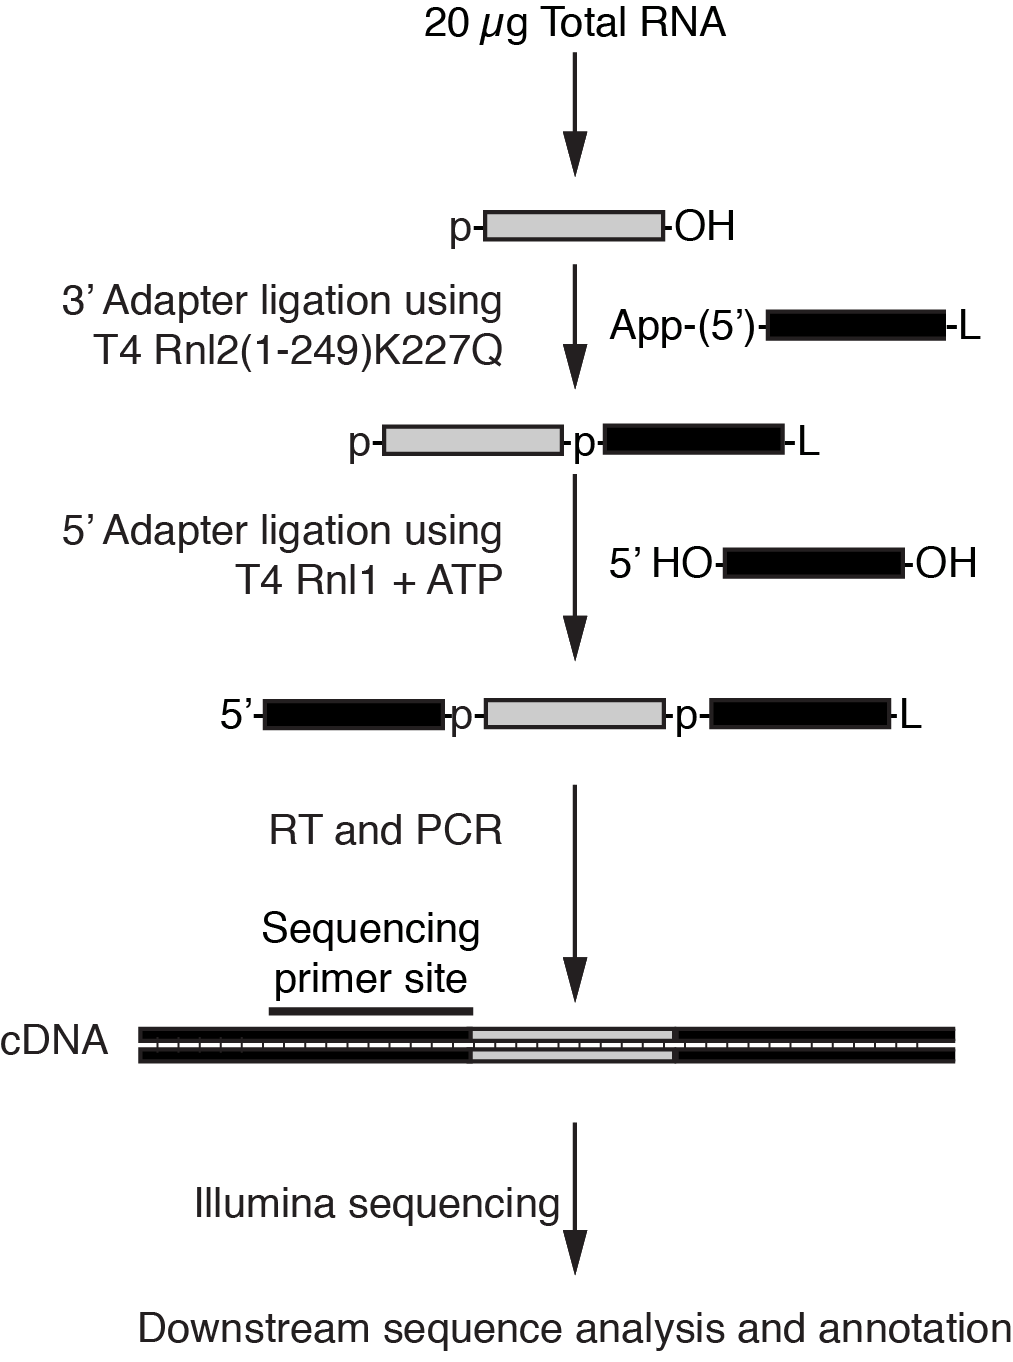
\includegraphics[width=3.5in]{sRNA.png}%
\caption[tRNA biogensis]{\textbf{Small RNA sequencing protocol.} thththtfahflahflahdflahdflahdfladfladhflasdhfladhfladhfladhfladhfaldjsfhaldskfjaldsfhalsdfhasdf}
\centering
\label{sRNA}%
\end{figure}

The utility of this protocol is documented for the discovery and study of miRNAs. Indeed, the decision to employ this protocol for sequencing of tRNAs is reasonable because:
\begin{itemize}
\item tRNAs, which are on average 75 nucleotides \cyan{nts} long are closer in length than most other ncRNAs (typically longer than 100 nts). 
\item mature tRNAs and miRNAs have a monophosphate at their 5' ends, which acts as the nucleophilic attacking group in the 5' ligation step. 
\end{itemize}
The application of this protocol for tRNA sequencing, though, resulting in \cyan{RNAseq} datasets with only \~2\% tRNA content, with an average length of 59 nts (\textbf{Fig. \ref{abysmal}}). These suggested that tRNAs were refractory to the small RNA sequencing protocol, and necessitated the development of a novel sequencing protocol. 

\begin{table}[!ht]
\begin{center}
\tabulinesep=1.2mm
\begin{tabu}{ | l | r | r |}
	\hline
    RNA type & \% Total reads & Mean length (nt) \\ \hline
	rRNA & 35.8\% & 60.5 \\ \hline
	no match  & 24.1\% & 76.2 \\ \hline
	no annotation & 17.8\% & 64.2 \\ \hline
	sn/snoRNA & 15.1\% & 62.5 \\ \hline
	repeat & 3.8\% & 59.1 \\ \hline
	tRNA & 2.0\% & 59.1 \\ \hline
	miscRNA & 1.3\% & 63.1 \\ \hline
	miRNA & 0.1\% & 22.2 \\
	\hline
\end{tabu}
\end{center}
\caption[RNA category from small RNA sequencing protocol]{\textbf{RNA category from small RNA sequencing protocol}}\label{abysmal}
\end{table}

\chapter{Results}

\section{Hydrolysis-based tRNA sequencing \cyan{(hydro-tRNAseq)}}
In order to overcome the problems associated with tRNA sequencing, we tried to identify the minimal number of simplest steps that could tackle the maximal number of problems. Thus, to curate 


\renewcommand{\bibname}{References}
%\bibliographystyle{IEEEtran}
\phantomsection
\printbibliography
\addcontentsline{toc}{chapter}{References} %rename references

\end{document}
